\chapter{轨迹与作图}
在前面的几章中,我们学习了直线形和圆的有关性质。
学习的途径主要是根据图形的定义和已知性质去推演图形的
其它性质。这一章,我们将把图形看成点的集合(点集),
研究如何根据点所具有的某种性质来求出点集在平面上的形
状和位置。

\section{轨迹}
\subsection{轨迹的概念}
我们知道,物体在运动中都要经过一定的路线。例如,
人在雪地里行走会留下明显的足迹,飞机飞行有一定的航
线,地球运行也有它的轨道等等。一般,我们常把物体按某
种规律运动的路线叫做物体运动的\textbf{轨迹}。在几何中,我们用
点表示物体在空间的位置。这样,一个点在空间按某种规律
运动的路线,我们就把它叫做这个点运动的轨迹,这个点就
叫做\textbf{动点}。例如,我们用圆规画圆时,圆规的一个脚尖固定
不动,而另一个脚上装上的铅笔尖端就可看作一个动点。它
和固定的脚尖保持一定的距离运动,所画出的图形就是这个
动点的轨迹。我们知道,圆是“同一平面上和某定点的距离
等于定长的点的集合”。由此可见,按某种规律运动的点的
轨迹,也就是具有某种性质的点的集合。

\begin{blk}{定义}
具有性质$\alpha$的所有点构成的集合,叫做具有性
质$\alpha$的点的轨迹。
\end{blk}

设$X=\{\text{具有性质$\alpha$的点}\}$。由上述定义,当我们要证明
某图形$A$是具有某种性质$\alpha$的点的轨迹时,也就是要证明
集合$A=X$. 要证明$A=X$, 就必须从以下两方面进行证
明:
\begin{enumerate}
\item $P$点$\in A\Rightarrow P$点具有性质$\alpha$ $(P\in X)$.
\item $P$点具有性质$\alpha$ $(P\in X)\Rightarrow P$点$\in A$.
\end{enumerate}

按上述两个方面证明,这是缺一不可的。如果我们只证
了第一条,实际上只是说明$A$是$X$的一个子集,并不能断
定$A=X$; 如果只证了第二条,也只是说$X$是$A$的一个子
集,同样不能断定$A=X$, 只有当我们证明了第一条:$A\subseteq
X$, 又证明了第二条:$X\subseteq A$, 我们才能断定$A=X$.

第一条证明了$A\subseteq X$, 这就是说在图形$A$上的点,都具
有性质$\alpha$. 没有一点是鱼目混珠的,通常把证这一条叫做证
\textbf{轨迹的纯粹性}。第二条证明了$X\subseteq A$, 这就是说,具有性质
$\alpha$的点都在图形$A$上,没有一点被遗漏掉。通常又把证这一
条叫做证\textbf{轨迹的完备性}。

由于原命题与逆否命题等价,所以也可以分别去证上述
两条的逆否命题,即要证轨迹的纯粹性也可证:
\[P\text{点不具有性质}\alpha\Rightarrow P\notin A\]
要证轨迹的完备性时,也可证:
\[P\text{点}\notin A\Rightarrow P\text{点不具有性质}\alpha\]

\begin{ex}
\begin{enumerate}
\item 叙
述两个集合相等的定义。
\item 在证轨迹命题时,为什么即要证轨迹的纯粹性,又要证
轨迹的完备性?
\item 如果我们证明了
$\overline{AB}$的垂直平分线上的任一点到$A$、
$B$两
点的距离相等,能否就说与$A$、$B$两点距离相等的点
的轨迹是$\overline{AB}$的垂直平分线?
\end{enumerate}
\end{ex}


\subsection{基本轨迹}
这一小节,我们来学习六个平面上的点的基本轨迹,我
们只证了1和4, 其它四个由同学们自证。

\begin{blk}{基本轨迹1}
与两个已知点距离相等的点的轨迹是连结
这两点的线段的垂直平分线。
\end{blk}

已知:两定点$A$、$B$, 直线$MN$是$\overline{AB}$的垂直平分线(图5.1)。

求证:与$A$、$B$两点距离相等的点的轨迹是直线$MN$.

\begin{figure}[htp]
    \centering
\begin{tikzpicture}[scale=.7]
\draw(-2,0)node[left]{$A$}--(2,0)node[right]{$B$};
\draw (0,3)node[above]{$M$}--(0,-2.5)node[below]{$N$};
\draw[dashed](-2,0)--(0,2.5)node[left]{$P$}--(2,0)--(0,-1.8)node[left]{$Q$}--(-2,0);
\node at (.25,.25){$O$};

\end{tikzpicture}
    \caption{}
\end{figure}


\begin{proof}
\begin{enumerate}
    \item 
设$P$是直线$MN$上的任一点,作$\overline{PA}$、$\overline{PB}$,
在$\triangle AOP$与$\triangle BOP$中,

$\because\quad \overline{AO}=\overline{BO},\quad \angle AOP=\angle BOP,\quad \overline{OP}=\overline{OP}$

$\therefore\quad \triangle AOP\cong \triangle BOP$ (SAS),
$\overline{PA}=\overline{PB}$.

这就说明了直线$MN$上的点,都与两点的距离相等。

\item 设$Q$为与$A$、$B$等距的点,即$\overline{QA}=\overline{QB}$. 过$AB$的
中点$O$与$Q$作直线$OQ$, 根据等腰三角形的性质,直线$OQ$
垂直平分$\overline{AB}$, 但$\overline{AB}$的垂直平分线只有一条,

$\therefore\quad MN$与$OQ$重合,$Q\in MN$.

\end{enumerate}

于是由1、2可知,与$A$、$B$两点距离相等的点的
轨迹是直线$MN$.
\end{proof}

\begin{blk}
{基本轨迹2} 与已知角的两边距离相等的点的轨迹是这
个已知角的平分线。
\end{blk}

\begin{blk}
{基本轨迹3} 与两条平行线等距离的点的轨迹是和这两
条平行线平行且平分它们的公垂线段的直线。
\end{blk}

\begin{blk}
    {基本轨迹4}与一条直线的距离等于定长的点的轨迹,是
    平行于这条直线,并和这条直线的距离等于定长的两条直线。
\end{blk}

已知:直线$CD\parallel$直线$AB$; 直线$EF\parallel$直线$AB$; $CD$、$EF$和$AB$之间的距离都是$d$(图5.2)。

求证:与$AB$的距离等于
$d$的点的轨迹是$CD$和$EF$.

\begin{figure}[htp]
    \centering
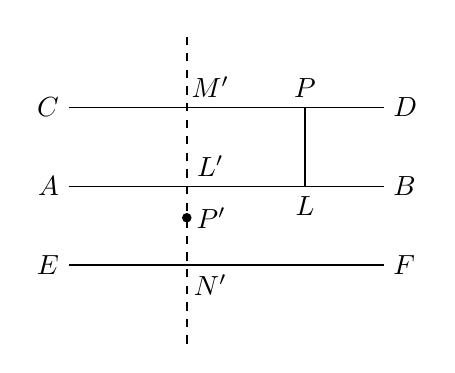
\begin{tikzpicture}
\draw (0,0)node[left]{$E$}--(4,0)node[right]{$F$};
\draw (0,1)node[left]{$A$}--(4,1)node[right]{$B$};
\draw (0,2)node[left]{$C$}--(4,2)node[right]{$D$};
\draw[dashed, thick] (1.5,-1)--(1.5,3);
\draw[thick] (3,1)node[below]{$L$}--(3,2)node[above]{$P$};
\node at (1.8,0)[below]{$N'$};
\node at (1.8,1)[above]{$L'$};
\node at (1.8,2)[above]{$M'$};
\draw (1.5,.6) [fill=black] circle (1.5pt) node[right]{$P'$};
\end{tikzpicture}
    
    \caption{}
\end{figure}


\begin{proof}
\begin{enumerate}
    \item 设$P$是$CD$或$EF$ 上的任一点。作$PL\bot AB$于$L$点。

$\because\quad CD\parallel AB$且和$AB$的距离等于$d$

$\therefore\quad \overline{PL}$是$AB$和$CD$的公垂线段,且$\overline{PL}=d$.

这就是说$CD$上的任一点和$AB$的距离都等于$d$, 同理
可证$EF$上的任一点和$AB$的距离也都等于$d$.
\item 设$P'$点是不在$CD$或$EF$上的任一点。
经过$P'$点作垂直于$AB$的直线,分别交$AB$、$CD$、$EF$于
$L'$、$M'$、$N'$, 则$\overline{M'L'}=\overline{N'L'}=d$.

$\because\quad P'$不在$CD$或$EF$上

$\therefore\quad P'$不和$M'$、$N'$重合

$\because\quad $在直线$M'N'$上和$L'$距离等于$d$的点只有$M'$、$N'$

$\therefore\quad \overline{P'L'}\ne d$

这就是说,不在$CD$和$EF$上的任何一点和$AB$的距离都
不等于$d$.
\end{enumerate}

于是由1、2可知,和$AB$的距离等于$d$的点的轨
迹是$CD$和$EF$。
\end{proof}

\begin{blk}
    {基本轨迹5} 与一个定点的距离等于定长的点的轨迹,
是以定点为圆心,定长为半径的一个圆。
\end{blk}

\begin{blk}
    {基本轨迹6}与一条定线段的两端连线所夹的角等于定角的点的轨迹,是以这条定线段为弦,所含的圆周角等于定
    角的两条弧。
\end{blk}

以上六个基本轨迹是研究其它轨迹问题的基础,同学们
一定要熟记。

\begin{example}
    求已知圆内等于定长的弦的中点的轨迹。

    已知$\odot (O,r)$和定长$a$, 且$a<2r$(图5.3)。

    求$\odot (O,r)$内等于定长$a$的弦的中点的轨迹。
\end{example}

\begin{figure}[htp]
    \centering
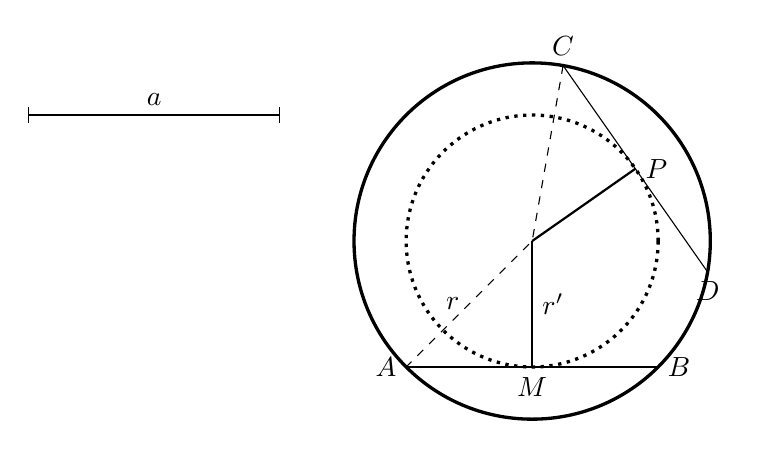
\begin{tikzpicture}[scale=1.6]
\draw[very thick] (0,0) circle (1.414)  ;  
\draw[very thick, dotted] (0,0) circle (1)  ;  
\draw (-45:1.414)node[right]{$B$}--(-45-90:1.414)node[left]{$A$};
\draw[dashed] (80:1.414)--(0,0)--node[left]{$r$}(-45-90:1.414);
\draw [thick] (0,0)--node[right]{$r'$}(0,-1)node[below]{$M$};
\draw (80:1.414)node[above]{$C$}--(-10:1.414)node[below]{$D$};
\draw [thick] (0,0)--(35:1)node[right]{$P$};

\draw[|-|](-4,1)--node[above]{$a$}(-2,1);
\end{tikzpicture}
    \caption{}
\end{figure}

\begin{solution}
    如图5.3, 设$\overline{AB}$是$\odot (O,r)$内等于定长$a$的弦,$M$
是它的中点,作$\overline{OM}$, 那么,$\overline{OM}\bot \overline{AB}$。
\[\overline{AM}=\frac{1}{2}\overline{AB}=\frac{a}{2}\]
所以
\[\overline{OM}=\sqrt{\overline{OA}^2-\overline{AM}^2}=\sqrt{r^2-\left(\frac{a}{2}\right)^2}\]
设$r'=\sqrt{r^2-\left(\frac{a}{2}\right)^2}$,则$r'$
为定长,以$O$为圆心,$r$为
半径画$\odot (O,r')$, 那么,$\odot (O,r)$内等于定长$a$的弦的中
点都在$\odot (O,r')$上。另外,在$\odot (O,r')$上任取一点$P$, 作
$\overline{OP}$, 再作弦$\overline{CD}\bot\overline{OP}$于$P$点,则$P$点是$\overline{CD}$弦的中点,且
\[\overline{CD}=2\overline{CP}=2\sqrt{r^2-{r'}^2}=2\sqrt{r^2-\left[r^2-\left(\frac{a}{2}\right)^2\right]}=2\cdot\frac{a}{2}=a\]
这就是说$\odot (O,r')$上的任一点都是$\odot (O,r')$内等于定长$a$
的一条弦的中点,所以我们所求的轨迹就是$\odot (O,r')$。
\end{solution}

\begin{example}
    过定圆外一定点引圆的割线,求割线被圆截下的弦的中点的轨迹。

    已知:定$\odot (O,r)$和$\odot O$外定点$P$(图5.4)。
    
    求:过$P$点引$\odot O$的割线,被$\odot O$截下的弦的中点
    的轨迹。
\end{example}


\begin{figure}[htp]
    \centering
\begin{tikzpicture}[scale=1.2]
\tkzDefPoints{0/0/O, 2.5/0/O', 5/0/P}
\draw[dashed] (P)--(-2,0)node[left]{$E'$};
\draw (0,0) circle (2);
\draw[dashed] (O') circle (2.5);
\tkzDefTangent[from with R=P](O, 2cm)
\tkzGetPoints{A}{B}
\tkzDrawSegments[add=0 and .2](P,A  P,B)
\node at (-.25,-.25){$O$};\node at (.25+2.5,.25){$O'$};
\node at (2.2,0)[above]{$E$};
\tkzDrawPoints(O',O)
\tkzDefShiftPoint[O'](150:2.5){M}
\tkzDefShiftPoint[O'](-142:2.5){N}
\tkzDefShiftPoint[O'](-155:2.5){X}
\tkzAutoLabelPoints[center=O'](M,N,X,A,B,P)
\tkzInterLC(P,M)(O,A) \tkzGetPoints{C'}{C}
\tkzInterLC(P,X)(O,A)\tkzGetPoints{D}{D'}
\tkzInterLC(P,N)(O,A)\tkzGetPoints{F}{F'}
\tkzAutoLabelPoints[center=O](D,F,C,C',D',F')
\draw(C')--(P)--(F');
\draw(D')--(P);
\draw[dashed](M)--(O)--(X);
\draw[dashed](A)--(O);
\end{tikzpicture}
    \caption{}
\end{figure}

\begin{solution}
    由于轨迹是具有某种性质$\alpha$的点的集合,求轨迹时,可先按照“性质”画出一些点,看看这些点可
能构成什么样的图形,如图
5.4, 过$P$点作$\odot O$的割线,与$\odot O$相交于$C$、$C'$, 作弦
$\overline{CC'}$的中点$M$, 我们证割线$PCC'$绕$P$点旋转,看这条变动
的割线被$\odot O$截下的弦的中点经过什么路线。大概可以看
出,可能是一段圆弧,究竟是不是圆弧,如果是圆弧,又如
何把它作出来,还要进一步分析。

$\because\quad M$是弦$\overline{CC'}$的中点,作$\overline{OM}$

则$\overline{OM}\bot\overline{CC'}$,即:$\angle OMP$是直角。

这就是说,过$P$点作$\odot O$的任一条 割线
被$\odot O$截下的弦的中点与$O$、$P$的连线的夹角等于直角,因
此,符合题中条件的弦的中点都在以$\overline{OP}$
为直径的圆上,以$\overline{OP}$
为直径作$\odot O'$, 我们所作的$\odot O'$是不是就是所求的轨迹呢?
这还要看$\odot O'$上有没有不符合条件的点。设$\odot O'$与$\odot O$相
交于$A$、$B$两点。显然,在$\odot O'$上$\wideparen{AOB}$外的点都是不合条
件的(包括$A$、$B$),我们再来看$\wideparen{AOB}$上的点是不是都是合
条件的点。在
$\wideparen{AOB}$上任取一点$X$, 设$PX$与$\odot O$相交于$D$、
$D'$, 作$\overline{OX}$, 则$\overline{OX}\bot \overline{DD'}$,所以$X$是$\overline{DD'}$的中点,这就
是说$\wideparen{AOB}$上的点都是过$P$点的某条割线被$\odot O$截下的弦的中
点。
\end{solution}

综合以上分析我们可得:过定圆外一定点引圆的割线,
割线被圆截下的弦的中点的轨迹是以定点与圆心间的线段为
直径的圆被夹在定圆内的一段弧。

\begin{ex}
    说出下列的点的轨迹是什么图形?并把它们分别画出
来。
\begin{enumerate}
    \item 到一条5cm长的线段的两端距离相等的点的轨迹。
    \item 通过两定点的圆的圆心的轨迹。
    \item 到一个等于60$^{\circ}$的已知角的两边距离相等的点的轨述:
    \item 与两条相交直线等距离的点的轨迹。
    \item 与$\angle AOB$的两边都相切的圆的圆心的轨迹。
    \item 与距离是3cm的两条平行直线$AB$、$CD$的距离相等的点
的轨迹。
\item 与距离是3cm的两条平行直线都相切的圆的圆心的轨
迹。
\item 和已知直线$AB$的距离等于2cm的点的轨迹。
\item 和已知直线$AB$相切,并且半径等于1.5cm的圆的圆心
的轨迹。
   \item 和一条已知直线切于已知点的圆的圆心的轨迹。
\item 与定点$A$的距离等于2cm的点的轨迹。
\item 和一条长是3cm的$AB$的两端连线所夹的角是直角的点
的轨迹。
\item 和一条长是4cm的已知线段$AB$的两端连线所夹的角等
于60$^{\circ}$的点的轨迹。

\end{enumerate}
\end{ex}


\section*{习题5.1}
\addcontentsline{toc}{subsection}{习题5.1}
\begin{enumerate}
    \item 求下列轨迹
\begin{enumerate}
    \item 以已知$\overline{AB}$为一边的三角形的外心的轨迹。
    \item 以已知$\overline{AB}$为一边,并且这边上的中线的长等于定长$m$的三角形的重心的轨迹。
\item 以3cm长的已知$\overline{AB}$为一边,并且面积等于6平方厘
米的三角形的顶点$C$的轨迹。
\item 和一个半径等于定长$r$的$\odot O$外切,并且半径等于
$r'$的圆的圆心的轨迹。
\item 以已知$\overline{BC}$为斜边的直角$\triangle ABC$的顶点$A$的轨迹。
\end{enumerate}

\item 叙述符合下列条件的点的轨迹。
\begin{enumerate}
    \item 平行于三角形的一边而夹在其余两边之间的线段的
中点的轨迹。
\item 平行于已知直线而在已知圆内的弦的中点的轨迹。
\end{enumerate}
\item 作出下列各题中给出的两个点集,向它们的交集各含有
几个元素。

\begin{enumerate}
    \item 和距离等于3cm的两条已知平行线$AB$、$CD$的距离
相等的点集;和直线$AB$上的一定点$E$的距离是2cm的点
集。
\item 和已知$\angle AOB$的两边的距离相等的点集;和边$OA$
的距离等于$d$的点集。
\item 和一条长3cm的已知$\overline{AB}$的两端连线所夹的角是直角
的点集;和$\overline{AB}$所在直线距离等于2cm的点集。
\end{enumerate}


\item 求通过$\odot (O,r)$内一定点$P$的弦的中点的轨迹。
\item 求到$\odot(O,3{\rm cm})$的圆面等于4cm的点的轨迹。
\end{enumerate}

\section{作图}
\subsection{基本作图}
在前几章中,我们曾用直尺、圆规解过不少作图题。在
这一节里,我们将进一步学习解作图题的一些重要方法,下
面列出我们已经学过的一些作图题(具体作法不再写出,由
同学自己复习、研究),这些作图题一般叫做\textbf{基本作图题},
它们是进一步解较复杂的作图题的基础。
\begin{enumerate}
\item 作一条线段等于已知线段,作一条线段等于$n$条线
段的和($n\ge 2$ 且 $n\in\mathbb{N}^+$)。
\item 作一条线段等于两条已知线段的差。
\item 作一个角等于已知角。
\item 平分一个已知角。
\item 过已知直线上或已知直线外一点,作已知直线的垂
线。
\item 作已知线段的垂直平分线。
\item 等分已知线段。
\item 按已知条件作三角形。
\begin{enumerate}
 \item 已知三边。
\item 已知两边及其夹角。
\item 已知两角及其中一角的对边。
\item 已知两角及其夹边。 
\end{enumerate}
\item 作三角形的外接圆和内切圆。
\item 已知斜边和一直角边,作直角三角形。
\item 已知线段$a$, 作一线段$x=\frac{m}{n}a$. (其中$\frac{m}{n}$
是正有理数)。
\item 作已知三条线段$a$、$b$、$c$的比例第四项。
\item 已知线段$a$、$b$, 作$a$、$b$的比例中项。
\item 已知线段$a$、$b$ $(a>b)$, 作线段$x=\sqrt{a^2+b^2}$
或$x=\sqrt{a^2-b^2}$。
\item 已知线段$a$, 作线段$x=\sqrt{\frac{m}{n}}a$ ($\frac{m}{n}$为正有理数)。
\item 过已知圆上一点作圆的切线。
\item 过已知圆外一点作圆的切线。
\item 作两个已知圆的公切线。
\item 过已知直线外的一个已知点,作这条直线的平行
线。
\end{enumerate}

\begin{ex}
\begin{enumerate}
    \item 作一直角三角形$ABC$, 使$\angle C=90^{\circ}$, $AB=3$cm, $BC=
    2$cm. 你能想出几种作法?
    \item 已知线段$a$、$b$,你能用几种方法作线段$x=\sqrt{ab}$。
    \item 已知线段$a$, 作线段$x=\sqrt{\frac{2}{3}a}$
        \item 过圆外一点,你能用几种方法作这个圆的切线。
\end{enumerate}
\end{ex}

\subsection{轨迹法作图}
我们在解作图题时,常常归结为要确定某些点的位置,
而这些点所要满足的条件又往往不是一个,我们只要根据点
所满足的各个条件,分别作出相应的轨迹,那么,这些轨迹
交集中的点,就是我们所要求作的点。

例如,已知两个定点$B$、$C$, 且
$\overline{BC}=3$cm (图5.5),以
$B$、$C$为两个顶点,求作一三角形,使第三个顶点与$B$的距
离是2cm, 与$C$的距离是4cm, 这个作图题,实际上就是确定
三角形的第三个顶点的位置。第三个顶点要满足两个条件:
\begin{enumerate}
    \item 和$B$点的距离是2cm
    \item 和$C$点的距离是4cm
\end{enumerate}
满足第一个条件的点的轨迹是$\odot(B,2{\rm cm})$,满足第二个条件的
点的轨迹是$\odot (C,4{\rm cm})$,所以第三个顶点就应该是$\odot(B,2{\rm cm})$与$\odot (C,4{\rm cm})$的交集中的点。由作图可知:
\[\odot(B,2{\rm cm})\cap \odot (C,4{\rm cm})=\{A, A'\}\]
于是,$A$点和$A'$点都是我们所
要求作的点,$\triangle ABC$与$\triangle A'BC$都是我们所要求作的三角
形。像这样应用轨迹的交集来确定点的位置,从而来解作图
题的方法,就叫做\textbf{轨迹法}。

\begin{figure}[htp]\centering
    \begin{minipage}[t]{0.48\textwidth}
    \centering
\begin{tikzpicture}[>=latex, scale=.8, rotate=-15]
\tkzDefPoints{0/0/B, 3/0/C, -.5/1.94/A,-.5/-1.94/A'}
\draw(A)--(B)--(C)--(A);
\draw(B)--(A')--(C);
\tkzDrawArc[delta=10](C,A)(A')
\tkzCompass(B,A)
\tkzCompass(B,A')
\tkzLabelPoints[above](A,C)
\tkzLabelPoints[left](A',B)

    \end{tikzpicture}
    \caption{}
    \end{minipage}
    \begin{minipage}[t]{0.48\textwidth}
    \centering
    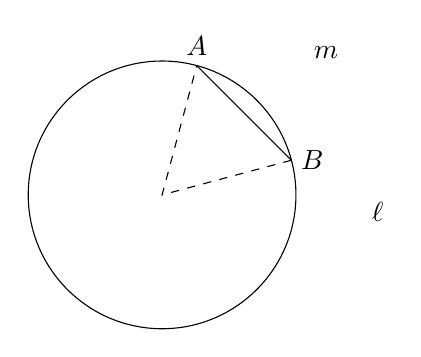
\begin{tikzpicture}[>=latex, scale=1.7]
\draw (0,0) circle(1);
\tkzDefPoints{0/0/O}
\tkzDrawPoints(O)
\tkzLabelPoints[below](O)
\tkzDefPoint(-5:1){C}
\tkzDefPoint(45:1){D}
\tkzDrawLines[add=.5 and .5](O,C O,D)
\draw[dashed](15:1)node[right]{$B$}--(0,0)--(75:1)node[above]{$A$};
\draw (75:1)--(15:1);
\node at (-5:1.5)[right]{$\ell$};
\node at (45:1.5)[right]{$m$};

    \end{tikzpicture}
    \caption{}
    \end{minipage}
    \end{figure}



\begin{example}
    已知一条定直线和直线外两个定点,求作一个
圆,使圆心在这条直线上,并且经过这两个定点。
\end{example}

已知:定直线$\ell$和两定点$AB$, 且$A\notin \ell$, $B\notin \ell$(图5.6)。

求作:一圆使圆心在$\ell$上,且经过$A$、$B$两点。

分析:假定$\odot O$为所求作的圆;那么,圆心$O$应满足两
个条件:
\begin{enumerate}
    \item $O\in \ell$;
    \item $O$点到$A$、$B$两点等距离。
\end{enumerate}
因为$\ell$
是已知的直线,而到$A$、$B$两点等距离的点的轨迹是$\overline{AB}$的
垂直平分线,所以,圆心$O$应是$\ell\cap \overline{AB}$的垂直平分线中的点,于是得作法如下:

作法:
\begin{enumerate}
\item 作$\overline{AB}$;
\item 作$\overline{AB}$的垂直平分线$m$与$\ell$相交于$O$点,
\item 以$O$为圆心,$OA$为半径作$\odot O$, 则$\odot O$即为所求
作的圆。
\end{enumerate}

\begin{proof}
    作$\overline{OA}$、$\overline{OB}$,

$\because\quad m$是$\overline{AB}$的垂直平分线,且$O\in m$.

$\therefore\quad \overline{OA}=\overline{OB}$

\begin{multicols}{2}
  $\because\quad A$点$\in \odot O$,

$\therefore\quad B$点$\in \odot O$,

又知$O$点$\in\ell$,

$\therefore \odot O$为所求作的圆。  
\end{multicols}

\end{proof}

讨论:
\begin{enumerate}
    \item 当直线$\ell$与AB所在的直线不垂直时,$\overline{AB}$的垂直平分线$m$与$\ell$一定有一个交点,且只有一个交点。这时,问
题有一解。
\item 当$\ell$与直线$\overline{AB}$垂直时,如果$\ell$与$m$重合时,问题
有无穷多解;如果$\ell\parallel m$时问题无解。
\end{enumerate}

\begin{example}
    已知三角形的一边和这条边上的中线及高,求作
三角形。
\end{example}

已知:线段$a$、$m$、$h$(图5.7)。

\begin{figure}[htp]
    \centering
\begin{tikzpicture}[scale=1.7]
\begin{scope}
    \draw(0,0)--node[above]{$h$}(1.4,0);
    \draw(0,.5)--node[above]{$m$}(1.6,.5);
    \draw(0,1)--node[above]{$a$}(2,1);
\end{scope}
\begin{scope}[xshift=3cm]
    

\draw(0,0)node[left]{$B$}--node[below]{$a$}(2,0)node[right]{$C$};
\draw(-.5,1.4)--(1.8,1.4);
\tkzDefPoints{1/0/M, 0.23/1.4/A}
\tkzCompass(M,A)
\draw(M)--node[right]{$m$}(A)--(2,0);
\draw(0,0)--(A)--node[right]{$h$}(0.23,0)node[below]{$D$};
\tkzLabelPoints[above](M,A)
\node (D) at (0.23,0){};
\tkzMarkRightAngle[size=.1](C,D,A)
\end{scope}
\end{tikzpicture}
    \caption{}
\end{figure}

求作:三角形使它的一边等于$a$, 且这边上的中线等于
$m$, 高等于$h$.

分析:画一草图(图5.7),假设$\triangle ABC$为所求作的三
角形,且$\overline{BC}=a$, $\overline{BC}$上的中线$\overline{AM}=m$, 高$\overline{AD}=h$, $B$、
$C$两个顶点由条件$\overline{BC}=a$, 很容易确定;$A$点的位置应该
满足条件:
\begin{enumerate}
    \item 与$\overline{BC}$的中点$M$的距离等于$a$的长;
    \item 与$\overline{BC}$所在直线的距离等于$h$.
\end{enumerate}
分别满足条件1和2的轨迹
都可作,故$A$的位置可作出,于是所要求作的三角形可作。

作法:(图5.8)
\begin{figure}[htp]
    \centering
\begin{tikzpicture}[scale=1.7]
    \draw(0,0)node[left]{$B$}--(2,0)node[right]{$C$};
\draw(-.5,1.4)--(2,1.4)node[right]{$\ell$};
\tkzDefPoints{1/0/M, 0.23/1.4/A}
\tkzCompass(M,A)
\draw(M)node[below]{$M$}--node[right]{$m$}(A)--(2,0);
\draw(0,0)--(A)--(0.23,0)node[below]{$D$};
\draw[dashed](1.5,0)--node[right]{$h$}(1.5,1.4);
\tkzLabelPoints[above](A)
\node (D) at (0.23,0){};
\tkzMarkRightAngle[size=.1](C,D,A)
\end{tikzpicture}
    \caption{}
\end{figure}

\begin{enumerate}
    \item 任取一点$B$, 作$\overline{BC}=a$,
    \item 作直线$\ell\parallel$直线$BC$,
    且与直线$BC$的距离等于$h$.
    \item 作$\overline{BC}$的中点$M$, 作$\odot(M,m)$交$\ell$于$A$点
    \item  作$\overline{AB}$、$\overline{AC}$, 则$\triangle
    ABC$为所求作的三角形。
\end{enumerate}

\begin{proof}
    (略)
\end{proof}

讨论
\begin{enumerate}
    \item 当$m\ge h$时,由于$\odot(M,m)$与直线$\ell$能够相
交,所以问题有一解。
\item 当$m<h$时,$\odot(M,m)$与直线$\ell$不相交,所以
这时问题无解。
\end{enumerate}

\begin{rmk}
    上题中所求作的三角形,并没有指定它在平面上
    的确切位置(叫做\textbf{不定位}),我们可在不同的位置分别作出很
    多满足已知条件的三角形,而且这些三角形都是全等形,遇到
    这种情况,我们任作一个满足条件的图形就可以了,并说问
    题只有一解;如果作出的满足已知条件的三角形不是全等
    形,那么要把这些图形都作出来,作出几个,我们就说问题
    有几解。如果在问题里是要求在固定位置作图(叫做\textbf{定位}),
    那么不管作出的是不是全等形,都要把它们作出来,作出几
    个我们就说问题有几解。 
\end{rmk}

\begin{example}
   求作和定角$\angle ABC$的两边都相切,并且半径等于
$r$的圆。 
\end{example}

已知:$\angle ABC$, 线段$r$(图5.9)。

求作:和$\angle ABC$的两边都相切,并且半径等于$r$的圆。

分析:画一草图(图5.10),假设$\odot O$为所求作的圆,
且$\odot O$的半径等于$r$, 那么圆心$O$应满足条件:
\begin{enumerate}
    \item 与$\angle ABC$的两边等距离;
    \item 与边$BA$或$BC$的距离等于$r$.
\end{enumerate}
满足1或2的轨迹都可作,故所求的圆的圆心可以作出。

作法:(图5.9)
\begin{enumerate}
    \item 作$\angle ABC$的平分线$BF$;
    \item 作直线$\ell\parallel BC$, 且与$BC$的距离等于$r$, 设$\ell$与$BF$
    相交于$O$点;
    \item 以$O$为圆心,$r$为半径作$\odot(O,r)$, $\odot(O,r)$即为所求作的圆。
\end{enumerate}

\begin{figure}[htp]\centering
    \begin{minipage}[t]{0.48\textwidth}
    \centering
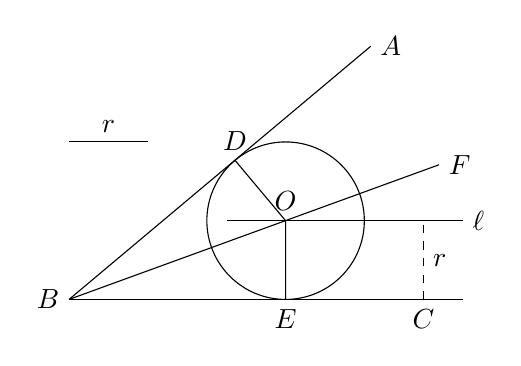
\begin{tikzpicture}[>=latex, scale=1]
\foreach \x in {0,20,40}
{
    \draw(0,0)--(\x:5);
}
\draw(2,1)--(5,1)node[right]{$\ell$};
\draw[dashed](4.5,0)node[below]{$C$}--node[right]{$r$}(4.5,1);
\draw(2.75,1) circle(1);
\draw(2.75,0)node[below]{$E$}--(2.75,1)node[above]{$O$}--(40:2.75)node[above]{$D$};
\node at (0,0) [left]{$B$};
\node at (20:5) [right]{$F$};
\node at (40:5) [right]{$A$};
\draw(0,2)--node[above]{$r$}(1,2);
    \end{tikzpicture}
    \caption{}
    \end{minipage}
    \begin{minipage}[t]{0.48\textwidth}
    \centering
    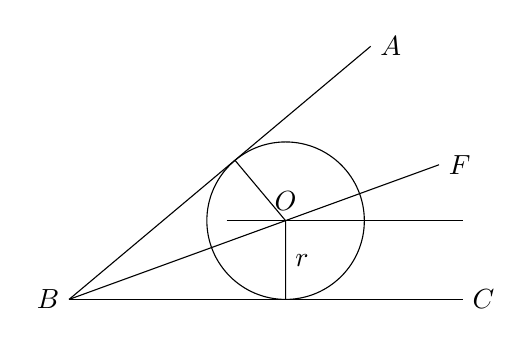
\begin{tikzpicture}[>=latex, scale=1]
\foreach \x/\xtext in {0/C,20/F,40/A}
{
    \draw(0,0)--(\x:5)node[right]{$\xtext$};
}
\draw(2,1)--(5,1);
\draw(2.75,1) circle(1);
\draw(2.75,0)--node[right]{$r$}(2.75,1)node[above]{$O$}--(40:2.75);
\node at (0,0) [left]{$B$};
\tkzDefPoint(40:2.75){D}
\tkzDefPoint(0:2.75){E}
\tkzDefPoint(2.75,1){O}\tkzDefPoint(0,0){B}
\tkzMarkRightAngles[size=.1](B,D,O B,E,O)


    \end{tikzpicture}
    \caption{}
    \end{minipage}
    \end{figure}

\begin{proof}
    作$\overline{OD} \bot BA$于$D$点,$\overline{OE}\bot BC$于$E$点。

$\because\quad EF$平分$\angle ABC$, 且$O\in BF$,

$\therefore\quad \overline{OD}=\overline{OE}$

又$\because\quad O\in\ell$, 而$\ell$与$BC$的距离是$r$的长。

$\therefore\quad \overline{OD}=\overline{OE}=r,\quad D\in \odot O,\quad E\in \odot O$

$\odot O$与$BA$和$BC$都相切,$\odot O$为所求作的圆。
\end{proof}

讨论:由于$\angle ABC$的平分线$BF$与直线$\ell$不会平行,所
以它们总有一个唯一的交点,所以此题只有一解。

从例5.5中可以看到,$\wideparen{DE}$把$\angle ABC$的两边在切点$D$、$E$
处连接起来了,这种连结叫做\textbf{直线与圆弧的平滑连接}。

\begin{example}
已知:$\odot (O_1,r_1)$和$\odot (O_2,r_2)$外离,且$r_1=
    10$mm, $r_2=8$mm(图5.11)。

    求作:一圆与$\odot (O_1,r_1)$外切,与$\odot (O_2,r_2)$内切,并
    且半径是20mm. 
\end{example}

\begin{figure}[htp]\centering
    \begin{minipage}[t]{0.48\textwidth}
    \centering
\begin{tikzpicture}[>=latex, scale=.7]
\draw (0,0) circle (2);
\draw (4,-1.2) circle (1.2);
\draw[thick](4,-3) circle (3);
\tkzDefPoints{0/0/O_1, 4/-1.2/O_2, 4/0/C1, 4/-3/O, 1.6/-1.2/B, 0/2/A, 1/-3/C}
\tkzLabelPoints[right](O_1,O_2,O)
\tkzLabelPoints(B,A,C)
\tkzDrawPoints(O_1,O_2,O, B,A,C)
\draw[dashed](O_1)--(O)--(4,0);
\tkzCompass(O_1,O)
\tkzCompass(C1,O)
    \end{tikzpicture}
    \caption{}
    \end{minipage}
    \begin{minipage}[t]{0.48\textwidth}
    \centering
    \begin{tikzpicture}[>=latex, scale=.5]
   \draw (0,0) circle (2);
\draw (4,-1.2) circle (1.2);
\draw[thick](4,-3) circle (3);
\tkzDefPoints{0/0/O_1, 4/-1.2/O_2, 4/-3/O}
\tkzLabelPoints[right](O_1,O_2,O)
\tkzDrawPoints(O_1,O_2,O)
\draw[dashed](O_1)--(O)--(4,0);   
    \end{tikzpicture}
    \caption{}
    \end{minipage}
    \end{figure}

\begin{analyze}
    画一草图(图5.12),设$\odot (O,20{\rm mm})$为要求作的
圆.由于$\odot (O,20{\rm mm})$与$\odot (O_1,r_1)$外切,并与$\odot (O_2,r_2)$内切,
所以
\[\begin{split}
   \overline{OO_1}&=r_1+20{\rm  mm}=30{\rm mm}\\
   \overline{OO_2}&=20{\rm  mm}-r_2=12{\rm  mm} 
\end{split}\]

因此,$O$点是$\odot (O_1,30{\rm mm})$和$\odot (O_2,12{\rm  mm})$的交点,
故$O$点可作出。
\end{analyze}

作法:(图5.11)。
\begin{enumerate}
    \item 作$\odot (O_1,30{\rm mm})$和$\odot (O_2,12{\rm mm})$, 设两圆有
交点$O$;
\item 以$O$为圆心,以20mm为半径作$\odot O$, 即$\odot O$为
所求作的圆。
\end{enumerate}

\begin{proof}
(略)
\end{proof}

讨论:
\begin{enumerate}
    \item 当$(r_1+20{\rm mm})+(20{\rm mm}-r_2)\ge \overline{O_1O_2}$时,
即当$ \overline{O_1O_2}\le 42{\rm mm}$时,问题有一解。
\item 当$ \overline{O_1O_2}> 42{\rm mm}$时,问题无解。
\end{enumerate}

从例5.6中的图5.11, 我们可看出$\odot O_1$的
$\wideparen{AB}$与$\odot O_2$的$\wideparen{BC}$
在切点$B$处连接起来了,这种连结叫做\textbf{圆弧与圆弧的平
滑连接}。

\begin{ex}
\begin{enumerate}
    \item 已知两定点$A$、$B$, 且直线$AB$与定直线$\ell$平行,在$\ell$上求作与$A$、$B$两点直线$\ell$距离相等的点。
    \item 求作和两条相交直线$\ell$和$m$的距离相等,且和它们的交点的距离等于定长$d$的点。
    \item 求作和已知直线$\ell$的距离等于定长$d$,并且和$\ell$上的一个定点的距离等于$2d$的点。
    \item 求作和$\overline{AB}$的两端的距离相等,且和$\overline{AB}$的两端的连线所夹的角等于定角$\alpha$的点。
    \item 求作等腰三
    角形,使它的底边等于定长$a$, 顶角等于定
    角$\alpha$.
    \item 求作一圆,使它的半径等于定长$a$, 且经过一定点并和
    一条定直线相切。
    \item 已知三角形的二边和其中一边上的高,求作三角形。
    \item 已知$\odot O(0,15{\rm mm})$和直线$\ell$, 并且$\ell$与$\odot O$相离,画半
    径为10mm的圆,使其与$\odot O$外切并和$\ell$相切。
\end{enumerate}
\end{ex}

\subsection{代数法作图}
解作图题时,有时也常常归结为要求作一条线段的长度
问题。这时我们可根据给出的条件,求出这条线段的代数表
达式,根据线段的代数表达式,把线段作出,使问题得到解
决。这种解作图题的方法,就叫做\textbf{代数分析法}。

\begin{example}
    已知:正方形$ABCD$(图5.13).

    求作:一点$P$使$P\in \overline{CD}$, 且$\overline{AP}=\overline{BC}+\overline{CP}$.
\end{example}

\begin{figure}[htp]\centering
    \begin{minipage}[t]{0.48\textwidth}
    \centering
\begin{tikzpicture}[>=latex, scale=1]
\tkzDefPoints{0/0/A, 0/2/D, 2/2/C, 2/0/B, 1/2/E, 1.5/2/P}
\tkzDrawPolygon(A,B,C,D)
\tkzLabelPoints[left](A,D)
\tkzLabelPoints[right](B,C)
\tkzLabelPoints[above](E,P)
\draw(A)--(P);
\tkzDrawPoints(E)
    \end{tikzpicture}
    \caption{}
    \end{minipage}
    \begin{minipage}[t]{0.48\textwidth}
    \centering
    \begin{tikzpicture}[>=latex, scale=1]
      \tkzDefPoints{0/0/A, 0/2/D, 2/2/C, 2/0/B,  1.5/2/P}
      \tkzDrawPolygon(A,B,C,D)
\tkzLabelPoints[left](A,D)
\tkzLabelPoints[right](B,C)
\tkzLabelPoints[above](P)
\draw(A)--(P);
\tkzDrawPoints(E)
    \end{tikzpicture}
    \caption{}
    \end{minipage}
    \end{figure}

\begin{analyze}
    画一草图(图5.14),已知正方形$ABCD$, 假设$P$点是所求作的点,即$P\in \overline{CD}$, 且$\overline{AP}=\overline{BC}+
    \overline{CP}$, 设
    $\overline{CP}=x$, $\overline{BC}=a$, 故$\overline{AP}=8+x$, $\overline{DP}=\overline{DC}-\overline{CP}=\overline{BC}-\overline{CP}=a-x$, 又因$\triangle ADP$是直角三角形,所以根据
    勾股定理有:$\overline{AP}^2=\overline{AD}^2+\overline{DP}^2$, 即:$(a+x)^2=a^2+(a-x)^2$.
    解此方程得
    $x=\frac{a}{4}$;$a$为已知,$\frac{a}{4}$
    可作出,故$P$点也可作
    出。
\end{analyze}

作法:(图5.13)。

\begin{enumerate}
    \item 作$\overline{CD}$的中点$E$.
    \item 作$\overline{CE}$的中点$P$, $P$点即为所求作的点。
\end{enumerate}

\begin{proof}
    由作图知$\overline{CP}=\frac{a}{4}$,

$\therefore\quad \overline{DP}=\overline{CD}-\overline{CP}=\frac{3}{4}a$
\[\overline{AP}=\sqrt{\overline{AD}^2+\overline{DP}^2}=\sqrt{a^2+\left(\frac{3}{4}a\right)^2}=\frac{5}{4}a=a+\frac{a}{4}\]
\[\overline{AP}=\overline{BC}+\overline{CP}\]
\end{proof}


讨论:由分析知,$\overline{DP}:\overline{PC}=3:1$, 因为分点$P$是唯一的,所以此题只有一解。


\begin{example}
    在已知线段上求作一点,分已知线段为两部分,
    使其中一部分是全线段和另一部分的比例中项。

    已知:$\overline{AB}$(图5.15).

    求作:$\overline{AB}$的内分点$G$, 使$\overline{AG}^2=\overline{AB}\cdot \overline{GB}$.
\end{example}

\begin{figure}[htp]\centering
    \begin{minipage}[t]{0.48\textwidth}
    \centering
\begin{tikzpicture}[>=latex, scale=.8]
    \draw(0,0)node[left]{$A$}--(0.618*4,0)node[below]{$G$}--(4,0)node[right]{$B$};
    \tkzDrawPoint(0,0)
    \tkzDrawPoint(0.618*4,0)
    \tkzDrawPoint(4,0)
\tkzDefPoints{4/2/D, 4/0/B, 0/0/A, 2.472/0/G}
\tkzDefPoint(26.57: 2.472){E}
\tkzDrawArc[delta=10](D,E)(B)
\tkzDrawArc[delta=10](A,G)(E)
\tkzDrawSegments(A,D D,B)
\tkzLabelPoints[above](D,E)

    \end{tikzpicture}
    \caption{}
    \end{minipage}
    \begin{minipage}[t]{0.48\textwidth}
    \centering
    \begin{tikzpicture}[>=latex, scale=1]
\draw(0,0)node[left]{$A$}--node[above]{$x$}(0.618*4,0)node[below]{$G$}--(4,0)node[right]{$B$};
\tkzDrawPoint(0,0)
\tkzDrawPoint(0.618*4,0)
\tkzDrawPoint(4,0)
    \end{tikzpicture}
    \caption{}
    \end{minipage}
    \end{figure}



\begin{analyze}
    画一草图(图5.16),已知$\overline{AB}$, 假定$G$为所求
    之点,设$\overline{AG}=x$, 则
    $\overline{BG}=a-x$,
    $x$满足方程
\[    x^2=a(a-x)\]
    即:$x^2+ax-a^2=0$. 解此方程得:
\[x_1=\frac{-a+\sqrt{4a^2+a^2}}{2},\qquad x_2=\frac{-a-\sqrt{4a^2+a^2}}{2}\quad \text{舍去}\]
$\therefore\quad x=\frac{-a+\sqrt{4a^2+a^2}}{2}=\sqrt{a^2+\left(\frac{a}{2}\right)^2}-\frac{a}{2}$

此线段$x$可作,故$G$点也可作出来。
\end{analyze}

作法:(图5.15)。
\begin{enumerate}
\item 作$\overline{ED}\bot\overline{AB}$, 使$\overline{BD}=\frac{1}{2}\overline{AB}$
\item 在$\overline{DA}$上截取$\overline{DE}=\overline{DB}$,\item 在$\overline{AB}$上截取$\overline{AG}=\overline{AE}$, $G$点即为所求作的点。
\end{enumerate}

\begin{proof}
    设$\overline{AB}=a$, 由作法有,
\[\begin{split}
    \overline{AG}&=\overline{AE}=\overline{AD}-\overline{ED}\\
&=\sqrt{\overline{AB}^2+\overline{BD}^2  }-\overline{BD}=\sqrt{a^2+\left(\frac{a}{2}\right)^2}-\frac{a}{2}\\
\overline{GB}&=\overline{AB}-\overline{AG}=a-\left(\sqrt{a^2+\left(\frac{a}{2}\right)^2}-\frac{a}{2}\right)\\
&=\frac{3}{2}a-\sqrt{a^2+\left(\frac{a}{2}\right)^2}
\end{split}\]
$\therefore\quad \overline{AB}\cdot \overline{GB}=a\left(\frac{3}{2}a-\sqrt{a^2+\left(\frac{a}{2}\right)^2}\right)$

由于:
\[\begin{split}
    \overline{AG}^2&=\left(\sqrt{a^2+\left(\frac{a}{2}\right)^2}-\frac{a}{2}\right)^2\\
&=a^2+\left(\frac{a}{2}\right)^2-2\x\frac{a}{2}\x \sqrt{a^2+\left(\frac{a}{2}\right)^2}+\left(\frac{a}{2}\right)^2\\
&=\frac{3}{2}a^2-a\sqrt{a^2+\left(\frac{a}{2}\right)^2}\\
&=a\left(\frac{3}{2}a-\sqrt{a^2+\left(\frac{a}{2}\right)^2}\right)
\end{split}
    \]
$\therefore\quad \overline{AG}^2=\overline{AB}\cdot \overline{BG}$

故$G$点为所求之点。
\end{proof}

讨论:由分析可知,满足条件的$\overline{AG}$总有一个,所以$G$
点总能作出一个,故此题有一解也只有一解。

由于
\[\overline{AG}=\sqrt{a^2+\left(\frac{a}{2}\right)^2}-\frac{a}{2}=\frac{\sqrt{5}}{2}a-\frac{1}{2}a=\frac{\sqrt{5}-1}{2}a\approx 0.618 a\]
所以$\overline{AG}$是$\overline{AB}$被$G$点分成的两段中,较长的一段,这种作图通常叫做分已知线段成“\textbf{中
外比}”,又叫做\textbf{黄金分割}。

\begin{example}
    在已知圆中,作内接正十边形。

已知:$\odot(O,r)$(图5.17).

求作:$\odot O$的内接正十边形。
\end{example}

\begin{figure}[htp]\centering
    \begin{minipage}[t]{0.48\textwidth}
    \centering
\begin{tikzpicture}[>=latex, scale=1]
\draw (0,0) circle (2.5);
\tkzDefPoint(0,0){O}
\foreach \x/\xtext in {0/D,1/E,2/F,3/G,4/H,5/I,6/J,7/A,8/B,9/C}
{
    \tkzDefPoint(\x*36:2.5){\xtext}
    \tkzDrawPoint(\xtext)
    \tkzAutoLabelPoints[center=O](\xtext)
}
\tkzDrawPolygon(A,B,C,D,E,F,G,H,I,J)
\draw(O)--(A);
\tkzDefPoint(-108:1.545){C'}  
\tkzLabelPoints[left](O, C') \tkzDrawPoints(O, C')
\tkzCompass[delta=10](A,B)
\tkzCompass[delta=10](B,C)
\tkzCompass[delta=10](C,D)
\tkzCompass[delta=10](D,E)
\tkzCompass[delta=10](E,F)
\tkzCompass[delta=10](F,G)
\tkzCompass[delta=10](G,H)
\tkzCompass[delta=10](H,I)
\tkzCompass[delta=10](I,J)
\tkzCompass[delta=10](J,A)
    \end{tikzpicture}
    \caption{}
    \end{minipage}
    \begin{minipage}[t]{0.48\textwidth}
    \centering
    \begin{tikzpicture}[>=latex, scale=.8]
        \draw (0,0) circle (2.5);
        \tkzDefPoint(0,0){O}
        \tkzDefPoint(7*36:2.5){A}
        \tkzDrawPoint(A)
        \tkzAutoLabelPoints[center=O](A)
        \tkzDefPoint(8*36:2.5){B}
        \tkzDrawPoint(B)
        \tkzAutoLabelPoints[center=O](B)
        \draw(O)--(A)--(B);
\tkzDefPoint(-108:1.545){C'}  
\tkzLabelPoints[left](O, C') \tkzDrawPoints(O, C')
\draw(C')--(B)--(O);
    \end{tikzpicture}
    \caption{}
    \end{minipage}
    \end{figure}







\begin{analyze}
    画一草图(图5.18),设$\overline{AB}$是$\odot O$的内接正十
边形的一边,则
\[\angle AOB=36^{\circ},\qquad \angle OAB=\angle OBA=72^{\circ}\]
作$\angle OBA$的平分线交$\overline{OA}$于$C'$点,则
\[\angle OBC'=\angle ABC'=\frac{1}{2}\angle OBA=36^{\circ}\]
又知$\angle BC'A=180^{\circ}-\angle ABC'-\angle OAB$,

$\therefore\quad \angle BC'A=72^{\circ},\quad 
\overline{OC'}=\overline{BC'}=\overline{AB}$, 且
$$\triangle OAE\backsim \triangle BAC',\quad \overline{OA}:\overline{AB}=\overline{AB}:\overline{AC'}$$

即:$\overline{AB}^2=\overline{OA}\cdot \overline{AC'}$

$\therefore\quad \overline{OC'}^2=\overline{OA}\cdot \overline{AC'}$
\end{analyze}

这个结果告诉我们,$C'$点恰好把半径$\overline{OA}$分成中外比且
$\overline{OC'}$是较长的一段。故应用黄金分割法由已知圆的半径作出
正十边形的边长,从而圆内接正十边形可以作出来。

作法 (图5.17).
\begin{enumerate}
\item 作半径$\overline{OA}$.
\item 作$C'$点分$\overline{OA}$成中外比,使$\overline{OC'}$为较长的一段,
\item 以$A$为起点,顺次作$\odot O$的弦$\overline{AB}$、$\overline{BC}$、$\overline{CD}$、
$\overline{DE}$、$\overline{EF}$、$\overline{FG}$、$\overline{GH}$、$\overline{HI}$、$\overline{IJ}$、$\overline{JA}$, 且使它们都
等于$\overline{OC'}$, 则$ABCDEFGHIJ$为所求作的圆内接正十边形。
\end{enumerate}



\begin{proof}
    (略)
\end{proof}

讨论:由分析可知一个圆内接正十边形的边长等于一个
定值,所以此问题有一解。

我们把圆十等分后,把相
间的五个分点用弦顺次连结,
就可作出圆内接正五边形,把
正五边形的五条对角线都作出
来,然后去掉各边剩下的图形
就是正五角星了(图5.19)。

\begin{figure}[htp]
    \centering
\begin{tikzpicture}[scale=.8]
\draw (0,0) circle (2.5);
\tkzDefPoint(0,0){O}
\foreach \x/\xtext in {0/A,1/B,2/C,3/D,4/E}
{
    \tkzDefPoint(18+\x*72:2.5){\xtext}
    \tkzDrawPoint(\xtext)
 %   \tkzAutoLabelPoints[center=O](\xtext)
}
\tkzDrawPolygon[dashed](A,B,C,D,E)
\tkzDrawSegments(A,C C,E B,D B,E A,D)

\foreach \x/\xtext in {0/A1,1/B1,2/C1,3/D1,4/E1}
{
    \tkzDefPoint(54+\x*72:2.5){\xtext}
   % \tkzAutoLabelPoints[center=O](\xtext)
}
\tkzCompass[delta=10](A,A1)
\tkzCompass[delta=10](A1,B)
\tkzCompass[delta=10](B,B1)
\tkzCompass[delta=10](B1,C)
\tkzCompass[delta=10](C,C1)
\tkzCompass[delta=10](C1,D)
\tkzCompass[delta=10](D,D1)
\tkzCompass[delta=10](D1,E)
\tkzCompass[delta=10](E,E1)
\tkzCompass[delta=10](E1,A)

\end{tikzpicture}
    \caption{}
\end{figure}


通过以上三例,我们看出,用代数法解作图题的一般步
骤:
\begin{itemize}
    \item 首先要分析解决这个问题需要作出哪条线段,并用$x$
表示;
\item 其次依照题中所给的条件和图形的性质,列出关于$x$
的方程;
\item 第三步,解这个方程(不合题意的根舍去);
\item 第四
步,依照方程的根的表示式,作出未知线段$x$; 
\item 第五步,完
成作图。即得所求作的图形。
\end{itemize}



\begin{ex}
\begin{enumerate}
    \item 已知线段$a$、$b$ ($a>b$), 求作下列线段$x$
\begin{multicols}{2}
    \begin{enumerate}
        \item $x=\frac{ab}{a+b}$
        \item $x=\sqrt{4a^2+b^2}$
        \item $x=\sqrt{a^2-\frac{b^2}{4}}$
        \item $x=\sqrt{a^2+3b^2}-\frac{b}{2}$
    \end{enumerate}
\end{multicols}
    \item 求作已知三角形的相似形,使它的面积等于已知三角形
    面积的三分之二。
    \item 从圆外一定点求作圆的一条割线,使它的圆外部分同圆
    内部分相等。
    \item 求作一正方形,使它同已知长方形等积。
    \item 在已知梯形中,求作底的平行线,平分已知梯形的面积。
    \item 作一圆的内接正五边形(只用尺、规)。
    \item 经过圆内一点作一条弦,使这个点是这条弦的一个三等
分点。
\end{enumerate}
\end{ex}


\section*{习题5.2}
\begin{enumerate}
    \item 已知线段$a$、$b$、$c$且$a>b$, 求作线段$x=\sqrt{a^2-b^2}+c$.
    \item 已知五条线段$a$、$b$、$c$、$d$、$e$, 求作线段$x=\frac{abc}{de}$。
    \item 已知线段$a$, 求作一条线段$x=\frac{\sqrt{5}-1}{2}a$
    \item 已知线段$a$、$b$, 且$a>b$, 求作$a+b$和$a-b$的比例中
    项。
    \item 求作与一个已知圆相切于已知点,且经过已知圆外的一
    个定点的圆。
    \item 已知三角形的一边长是3cm, 这边上的中线长4cm, 这边
    的对角是$65^{\circ}$, 求作这个三角形。
    \item 已知一边和这边上的中线及另一边上的高线,求作这个
    三角形。
    \item 求作一个三角形,使它同已知三角形等积,又同另一个
    已知的三角形相似。
    \item 求作直径是$d$的圆内接矩形,使它的面积等于每边是$a$
    的已知正方形面积(提示:设矩形的长、宽各为$x$、$y$,
    列出含有$x$、$y$的方程组解之)。
    \item 从已知圆外的一个已知点,作圆的割线,使它在圆外的
    部分与圆内的部分的比是$1:2$.
    \item 求作过两定点,且在一条定直线上截取定长弦的圆
    (提示:利用切割线定理)。
\end{enumerate}

\section*{复习题五}

\begin{enumerate}
    \item 连结一定直线上的点和线外一定点的线段,求这线段中
    点的轨迹。
    \item 求具有公共底边,且这边上的高相等的三角形顶点的轨
    迹。
    \item 三定点$A$、$B$、$C$在一直线上,且$\overline{AB}=\overline{BC}$, 求与$A$、$B$
    两点和与$B$、$C$两点连线夹角相等点的轨迹。
    \item 从一定点$A$向通过另一定点$B$的动直线引垂线,求垂足
    $P$的轨迹。
    \item 求到两定点$A$、$B$的距离的平方和等于$\overline{AB}^2$
    的点的轨迹。
    \item 求到一定圆引切线,切线长等于定长的点的轨迹。
    \item 求对相交的两定圆有等幂的点的轨迹。
    \item 求到两定点$A$、$B$平方差等于$\overline{AB}^2$的点的轨迹。
    \item 已知三点$A$、$B$、$C$在一条直线上,求与$A$、$B$两点和$B$、
   $ C$两点连线夹角相等的点的轨迹。
    \item 求作一个圆使和两条已知平行线都相切,并且经过两平
    行线间一个已知点。
    \item 已知$\odot(O_1,1.5{\rm cm})$, $\odot(O_2,1{\rm cm})$, 圆心间的距离
    $\overline{O_1O_2}=4{\rm cm}$, 求作一圆,使它的半径等于1.3cm, 并且
    和$\odot O_1$与$\odot O_2$都外切。
    \item 已知$\odot(O_1,1.4{\rm cm})$, $\odot(O_2,1{\rm cm})$, $\overline{O_1O_2}=3{\rm cm}$, 求
    作一个圆,使它的半径为3.2cm, 并且和$\odot O_1$与$\odot O_2$都相内切。
    \item 已知线段$a$, 求作线$x=\sqrt{3a}$, $y=\sqrt{12a}$.
    \item 已知线段$x$与$y$满足方程组:
    \[\begin{cases}
        \frac{x+y}{2}=a\\
        \sqrt{xy}=b
    \end{cases}\qquad (a>b)\]
    求作线段$x$和$y$. 
    \item 作一个三角形具有已知的周长,并和一个已知三角形相
似。
\item 求作$\triangle ABC$的内接正方形,使正方形的一边位于$\overline{AB}$边
上,另外两个顶点各在$\overline{AC}$边和$\overline{BC}$边上。
\item 在已知正方形$ABCD$内作内接正方形,使内接正方形的
四个顶点分别在正方形的各边上,且使它的边长等于定
长$b$.
\item 把任一个三角形改为等边三角形,使它的面积不变。
\item 求作三个两两外切的圆,使它们的半径分别等于1cm,
 2cm, 3cm.
\item 作一个正五角星(只画出图形).
\item 已知$A$、$B$、$C$为定直线$\ell$上的三个定点,求作$\odot A$、
$\odot B$、$\odot C$使它们两两均相切,但不切于同一点。
\item 在已知矩形内作两个互相外切的等圆,使各切于这矩形
一组对角的两边。
\end{enumerate}
